
\documentclass[11pt,fleqn]{article} 
\usepackage[margin=0.8in, head=0.8in]{geometry} 
\usepackage{amsmath, amssymb, amsthm}
\usepackage{fancyhdr} 
\usepackage{palatino, url, multicol}
\usepackage{graphicx, pgfplots} 
\usepackage[all]{xy}
\usepackage{polynom} 
%\usepackage{pdfsync} %% I don't know why this messes up tabular column widths
\usepackage{enumerate}
\usepackage{framed}
\usepackage{setspace}
\usepackage{array,tikz,hyperref,tikz-3dplot}

\pgfplotsset{compat=1.6}

\pgfplotsset{soldot/.style={color=black,only marks,mark=*}} \pgfplotsset{holdot/.style={color=black,fill=white,only marks,mark=*}}


\pagestyle{fancy} 
\lfoot{}
\rfoot{\S 2.2}

\begin{document}
\renewcommand{\headrulewidth}{0pt}
\newcommand{\blank}[1]{\rule{#1}{0.75pt}}
\newcommand{\bc}{\begin{center}}
\newcommand{\ec}{\end{center}}
\renewcommand{\d}{\displaystyle}

\vspace*{-0.7in}

%%%%%%%%%intro page
\begin{center}
  \large
  \sc{Section 2.2: Volumes by Slicing}\\
\end{center}
Start by showing students the cross-section demonstration and the volume by rotation demonstration.
\begin{itemize}
	\item \href{https://uaf-math.github.io/calc2/assets/worksheets/F25/M252_2_2_demo_cross_section.html}{A Solid Defined by Cross-Sections}
	\item \href{https://demonstrations.wolfram.com/SolidsOfRevolution/}{Solids Defined by Rotation}
\end{itemize} 
\begin{enumerate}
\item Translating our Calculus I calculations of Area to Volumes.\\

\vfill


% Set the 3D plotting parameters for perspective
% for the cone
\tdplotsetmaincoords{70}{110}
\begin{tikzpicture}[tdplot_main_coords, scale=2]
% Define some colors
\definecolor{conecolor}{rgb}{0.8,0.6,0.2}

% Draw the cone
\begin{scope}
    % Cone base (ellipse in perspective)
    \draw[fill=conecolor!30, draw=conecolor!80] 
        plot[domain=0:360, samples=60] 
        ({cos(\x)}, {sin(\x)}, 0);
    
    % Cone surface (using parametric approach)
    \foreach \angle in {0,10,...,350} {
        \draw[conecolor!60, opacity=0.3] 
            ({cos(\angle)}, {sin(\angle)}, 0) -- (0, 0, 2);
    }
    
    % Cone apex
    \filldraw[conecolor!80] (0, 0, 2) circle (0.02);
    
    % Cone outline (visible edges)
    \draw[thick, conecolor!90] (1, 0, 0) -- (0, 0, 2);
    \draw[thick, conecolor!90] (-1, 0, 0) -- (0, 0, 2);
    \draw[thick, conecolor!90] (0, 1, 0) -- (0, 0, 2);
    \draw[thick, conecolor!90] (0, -1, 0) -- (0, 0, 2);
\end{scope}
\end{tikzpicture}
\hfill
Skate Park Ramp
\tdplotsetmaincoords{50}{-10}
\begin{tikzpicture}[tdplot_main_coords, scale=2]
\definecolor{rampcolor}{rgb}{0.2,0.6,0.8}
% Draw the curved ramp
\begin{scope}[shift={(3, 0, 0)}]
    % Ramp surface - curved in 3D
    \foreach \t in {0,0.1,...,2} {
        \pgfmathsetmacro{\x}{\t}
        \pgfmathsetmacro{\z}{0.5*\t*\t}  % Quadratic curve for height
        \pgfmathsetmacro{\nextx}{\t+0.1}
        \pgfmathsetmacro{\nextz}{0.5*(\t+0.1)*(\t+0.1)}
        
        % Draw cross-sections of the ramp
        \draw[rampcolor!40, fill=rampcolor!20] 
            (\x, -0.5, \z) -- (\x, 0.5, \z) -- 
            (\nextx, 0.5, \nextz) -- (\nextx, -0.5, \nextz) -- cycle;
    }
    
    % Ramp edges (front curves)
    \draw[thick, rampcolor!90] 
        plot[domain=0:2, samples=20] 
        (\x, -0.5, {0.5*\x*\x});
    \draw[thick, rampcolor!90] 
        plot[domain=0:2, samples=20] 
        (\x, 0.5, {0.5*\x*\x});
    
    % *** ADDED: Back edges of ramp (dashed to show they're behind) ***
    \draw[thick, rampcolor!60, dashed] 
        plot[domain=0:2, samples=20] 
        (\x, -0.5, 0);  % Back bottom edge
    \draw[thick, rampcolor!60, dashed] 
        plot[domain=0:2, samples=20] 
        (\x, 0.5, 0);   % Back top edge
    
    % *** ADDED: Vertical back edges connecting bottom to curved top ***
    \foreach \x in {0.5, 1.0, 1.5,2} {
        \pgfmathsetmacro{\z}{0.5*\x*\x}
        \draw[thick, rampcolor!60, ultra thick] (\x, -0.5, 0) -- (\x, -0.5, \z);
        \draw[thick, rampcolor!60, dashed] (\x, 0.5, 0) -- (\x, 0.5, \z);
    }
    
    % End faces
    \draw[thick, rampcolor!90, fill=rampcolor!30] 
        (0, -0.5, 0) -- (0, 0.5, 0) -- (0, 0.5, 0) -- (0, -0.5, 0) -- cycle;
    \draw[thick, rampcolor!90, fill=rampcolor!30] 
        (2, -0.5, 2) -- (2, 0.5, 2) -- (2, 0.5, 2) -- (2, -0.5, 2) -- cycle;
    
    % Bottom of ramp (front edges)
    \draw[thick, rampcolor!70] (0, -0.5, 0) -- (2, -0.5, 0);
    \draw[thick, rampcolor!70] (0, 0.5, 0) -- (2, 0.5, 0);
\end{scope}

% Add ground plane for reference
%\draw[gray!30, very thin] (-2, -2, 0) grid (6, 2, 0);

%% Add coordinate axes for reference
%\draw[->] (0,0,0) -- (1.5,0,0) node[anchor=north east]{$x$};
%\draw[->] (0,0,0) -- (0,1.5,0) node[anchor=north west]{$y$};
%\draw[->] (0,0,0) -- (0,0,1.5) node[anchor=south]{$z$};

\end{tikzpicture}


\item A general formula for volume using slices:

\vspace{1.5in}
\newpage
\item Sketch the region $R$ bounded by $y=\sqrt{x}$, $y=0$, and $x=4.$ Determine the volume of the solid with cross-sections perpendicular to the base and parallel to the $y$-axis are squares.\\
\vfill

\item Sketch the same region as in problem 1 above (i.e. the region $R$ bounded by $y=\sqrt{x}$, $y=0$, and $x=4$). Find the volume of the solid obtained by rotating this region about the $x$-axis. Attempt to describe and/or draw what this solid looks like.\\

\vfill

\item The Disk Method

\vspace{1.5in}
\newpage
\item On the axes below, sketch and shade the region bounded by $y=x^{2/3}$, $x=0$ and $y=1.$ Then below, sketch the solid obtained by rotating this region about the {\Large{$y$-axis}}.  \textbf{Set up} an integral to calculate the volume of the solid. Include your sample slice. Evaluate this integral once your have completed the rest of the sheet.\\

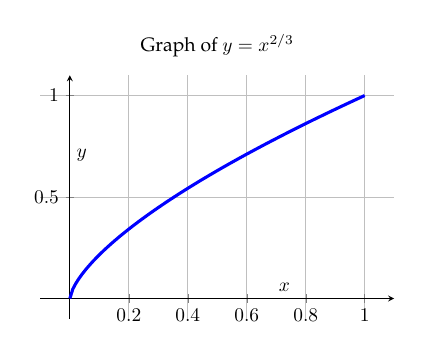
\begin{tikzpicture}[scale = .7]
\begin{axis}[
    xlabel={$x$},
    ylabel={$y$},
    title={Graph of $y = x^{2/3}$},
    domain=0:1,
    samples=100,
    grid=major,
    axis lines=middle,
    enlargelimits=true,
    width=8cm,
    height=6cm
]
\addplot[blue, ultra thick] {x^(2/3)};
\end{axis}
\end{tikzpicture}
\vfill
\item Sketch, label, and shade the region bounded by $y=\sqrt{x}$ and $y=x^2$. In another place, sketch the solid obtained by rotating this region about the $x$-axis.  \textbf{Set up} an integral to calculate the volume of the solid. Include your sample slice. Evaluate this integral once your have completed the rest of the sheet.\\


\vfill
\newpage
\item The Washer Method

\vspace{2in}


\item Find the volume of the solid obtained by rotating about the $y$ axis the region bounded by $y=x^2$ and $y=4x.$ (Sketch the region. Draw a slice.)
\vfill
\end{enumerate}
\end{document}

